\documentclass{beamer}
\usepackage[utf8]{inputenc}

\usetheme{Madrid}
\usecolortheme{default}
\usepackage{amsmath,amssymb,amsfonts,amsthm}
\usepackage{txfonts}
\usepackage{tkz-euclide}
\usepackage{listings}
\usepackage{adjustbox}
\usepackage{array}
\usepackage{tabularx}
\usepackage{gvv}
\usepackage{lmodern}
\usepackage{circuitikz}
\usepackage{tikz}
\usepackage{graphicx}

\setbeamertemplate{page number in head/foot}[totalframenumber]

\usepackage{tcolorbox}
\tcbuselibrary{minted,breakable,xparse,skins}



\definecolor{bg}{gray}{0.95}
\DeclareTCBListing{mintedbox}{O{}m!O{}}{%
  breakable=true,
  listing engine=minted,
  listing only,
  minted language=#2,
  minted style=default,
  minted options={%
    linenos,
    gobble=0,
    breaklines=true,
    breakafter=,,
    fontsize=\small,
    numbersep=8pt,
    #1},
  boxsep=0pt,
  left skip=0pt,
  right skip=0pt,
  left=25pt,
  right=0pt,
  top=3pt,
  bottom=3pt,
  arc=5pt,
  leftrule=0pt,
  rightrule=0pt,
  bottomrule=2pt,
  toprule=2pt,
  colback=bg,
  colframe=orange!70,
  enhanced,
  overlay={%
    \begin{tcbclipinterior}
    \fill[orange!20!white] (frame.south west) rectangle ([xshift=20pt]frame.north west);
    \end{tcbclipinterior}},
  #3,
}
\lstset{
    language=C,
    basicstyle=\ttfamily\small,
    keywordstyle=\color{blue},
    stringstyle=\color{orange},
    commentstyle=\color{green!60!black},
    numbers=left,
    numberstyle=\tiny\color{gray},
    breaklines=true,
    showstringspaces=false,
}
\title 
{MatGeo Assignment 1.11.9}

\author
{AI25BTECH11007}
\begin{document}

\frame{\titlepage}
\begin{frame}{Question}
If
\[
\vec{a} = \hat{i} - 7\hat{j} + 7\hat{k}
\quad \text{and} \quad
\vec{b} = 3\hat{i} - 2\hat{j} + 2\hat{k},
\]
find a unit vector perpendicular to both the vectors $\vec{a}$ and $\vec{b}$.\\
\end{frame}
\begin{frame}{Solution}

A vector perpendicular to both $\vec{a}$ and $\vec{b}$ is given by
\[
\vec{n} = \vec{a} \times \vec{b}.
\]

\[
\vec{n} =
\begin{vmatrix}
\hat{i} & \hat{j} & \hat{k} \\
1 & -7 & 7 \\
3 & -2 & 2
\end{vmatrix}.
\]

Expanding,
\[
\vec{n} = \myvec{0 \\ 19 \\ 19}.
\]

The magnitude is
\[
|\vec{n}| = \sqrt{0^2 + 19^2 + 19^2} = 19\sqrt{2}.
\]
\end{frame}
\begin{frame}
Hence the required unit vector is
\[
\hat{n} = \frac{\vec{n}}{|\vec{n}|}
= \frac{1}{19\sqrt{2}} \myvec{0 \\ 19 \\ 19}
= \myvec{0 \\ \tfrac{1}{\sqrt{2}} \\ \tfrac{1}{\sqrt{2}}}.
\]

Therefore, a unit vector perpendicular to both $\vec{a}$ and $\vec{b}$ is
\[
\hat{n} = \frac{1}{\sqrt{2}}(\hat{j} + \hat{k}),
\]
or its negative.

\end{frame}


\begin{frame}{Plot}
    \begin{figure}[H]
    \centering
    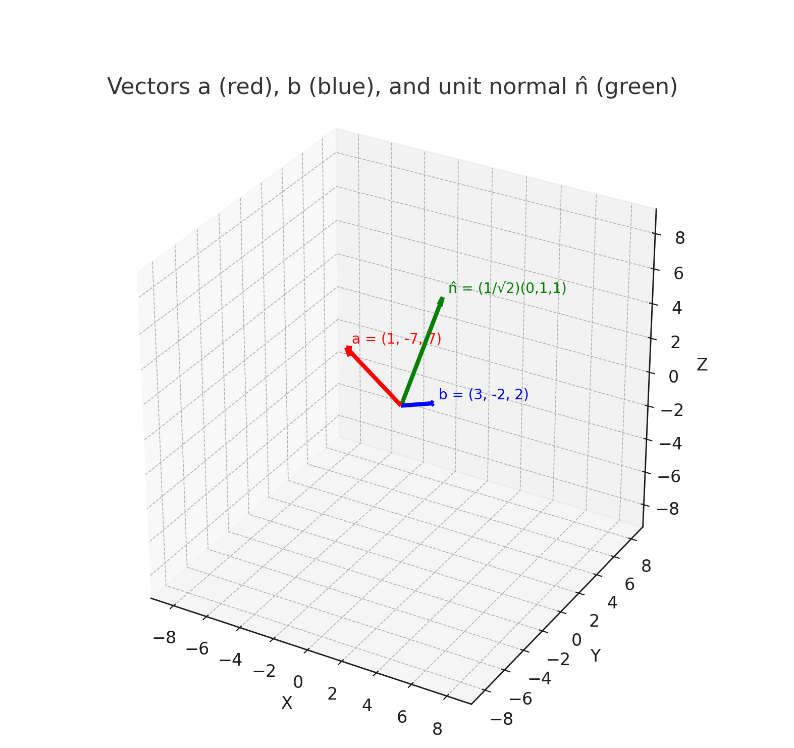
\includegraphics[width=0.75\columnwidth]{figs/image.png}
    \caption{Image Visual}
    \label{fig:figs/image.png}
    \end{figure}
\end{frame}

\begin{frame}{Conclusion}
    Therefore, a unit vector perpendicular to both $\vec{a}$ and $\vec{b}$ is
\[
\hat{n} = \frac{1}{\sqrt{2}}(\hat{j} + \hat{k}),
\]
or its negative.
\end{frame}
\end{document}